\chapter{Approche modulaire des réseaux de neurones}
\graphicspath{{01-Modularite/}}

\minitoc
%%%%%%%%%%%%%%%%%%%%%%%%%
% Intro du chapitre : Trouver un questionnement, un exemple qui parle de modularité dans les systèmes biologiques:  
% se placer dans le contexte de 
% - modularité : finalement on ne sait pas trop ce que c'est 
% - apprentissage ! 
% - réseaux de neurones
%%%%%%%%%%%%%%%%%%%%%%%%%

\section{Contexte}
L'idée de ce chapitre est d'inscrire nos travaux dans le coté modulaire des réseaux de neurones. Il nous foudra donc définir proprement ce qu'on appelle modularité, et définir les motivations pour créer une architecture modulaire. Il faut def ce qu'on appelle réseau de neurones et apprentissage automatique. 

D'une part, de nombreux modèles biologiques présentent des architectures modulaires. Notre conception du monde se présente en fait sous une forme de modularité. En tant qu'humain, nous comprenons le monde de notre point de vue, en le décomposant pour qu'il semble accessible : en effet notre raisonnement est modulaire, notre système social, groupes d'individus, etc, comme l'explique par exemple \cite{Morowitz1995TheMT} dans "How a mind resides in the brain".
Nos contructions sont modulaires : programme informatique ... Il est difficile de concevoir et surtout de comprendre, en tant qu'humain, un système qui ne serait pas décomposable en modules. Prenons comme exemple les réseaux de neurones profonds : la compréhension  et l'interprétabilité ces programmes est un défi de la recherche actuelle. Pour cette interprétation, on cherche des éléments symboliques, des groupes, des communautés. 
La décomposition des sciences elles même, par exemple, nous permet de trouver des solutions aux problèmes a des échelles différentes. Le programmeur n'a pas besoin de comprendre en profondeur quels transistors composent les circuits; l'expert.e en electronique n'a pas besoin de d'abord résoudre les équations qui régissent les mouvements ioniques au sein des transistors pour concevoir des circuits, etc. Seuls les principes régissant les comportement globaux d'un système commme le transistors ont besoins d'être connus pour utiliser ces sytèmes dans une tâche; tâche qui consituera également un module dans son ensemble et qui sera régie par des principes généraux, du transitor à l'utilisation d'un logiciel de dessin. 
Mais est ce que cette hiérarchie modulaire est essentiellement subjective ? A priori non. Une organisation modulaire est présente et calculable dans de nombreux systèmes.


Présentation d'exemples de théories dérivées d'une modularité bio-inspirée. 
Brooks \cite{brooks_sumsumption_85}

Les modules sont également associés aux systèmes complexes. De nombreux travaux sont ainsi réalisés à la frontière entre domaines, 
Réseaux associés aux systèmes complexes, interactions.


\subsection{Systèmes complexes}


Argument : les systèmes complexes montrent des propriétés d’emergence de comportement. Statiquement, cela peut etre la contruction de fractales, ou dynamiquement des systèmes régis par des équations non linéaires. Ex synchronisation dans les réseaux : lucioles, oiseaux, et surtout cerveau. L’émergence de propriétés est difficile a prédire et exprimer par la nature des systèmes. un système complexe s’étudie en effet en le simulant. On a l’état initial et les équations qui régissent la dynamique (passage d’un état a un autre, ou en version continue), mais il est trop commpliqué d’exprimer sous forme d’équation un état courant. 
Il est donc judicieux d’explorer et de simuler des nouveaux systèmes complexes, car on ne peut pas vraiment prédire d’ores et déjà un comportement. 

→ Auto-organisation definition

Les phénomènes d’auto-organisation sont déjà un élément caractéristique des systèmes complexes : Alan Turing montre qu’a partir d’un état presque uniforme de composants chimique, leur réaction et diffusion crée des motifs répétés. Ces motifs sont créés a partir de règles locales, on est bien sur un phénomène auto-organisé. Plus surprenant ces motifs appelés “turing patterns” sont présents dans de nombreux systèmes biologiques, par exemple sur la peau des animaux. Cela montre la prévalence des phénomènes d’auto-organisation dans la nature. 

A partir de règles locales, des comportements globaux peuvent donc émerger, de façon auto-organisée. Un des exemples biologiques montrant cette complexité est ainsil le cerveau humain. 



%Les systèmes, dans leur échelles, sont donc complexes. Si on peut décomposer des systèmes pour les étudier, ils restent liés au sein d'un vaste écosystème. Ainsi, l'étude de la modularité des systèmes est présente au sein des approches biologiques.
%"Un système complexe est un ensemble constitué d'un grand nombre d'entités en interaction dont l'intégration permet d'achever une mission commune. L'étude de ce type de système ne peut passer que par la simulation.
%Les systèmes complexes sont caractérisés par des propriétés émergentes qui n'existent qu'au niveau du système et ne peuvent pas être observées au niveau de ces constituants.
%(wikipedia)". Ces constituants interagissent par des règles locales qui sont souvent simples, mais dont l'interaction forme des propriétés émergentes. Complexe ne veut pas dire que les relations et interactions sont difficiles a exprimer : un système est complexe du point de vue d'un observateur, mais les règles locales sont souvent simples. Des exemples de systèmes complexes sont ainsi le comportement de fourmis au sein d'une fourmilière, le comportement des oiseaux en nuée, les réseaux sociaux, l'interaction entre protéines, les réseaux de neurones biologiques dans le cerveau.
%
%L'Emergence de motifs et de phénomènes d'auto-organisation (turing patterns) \cite{turing52} sont même utilisés pour qualifier le système complexe. En 1952, Alan turing montre que dans un système chimique comprenant de la réaction entre éléments et de la diffusion, des motifs spatiaux émergent, a partir de conditions initiales presque uniforment. Ces motifs se retrouvent dans de nombreux systèmes, chimique ou non.
%
%Il n'y a a priori pas de définition commune concernant ce qu'on appelle un système complexe et comment le mesurer. On pourrait plutot voir la complexité comme une façon d'étudier un objet. Un exemple de définition de la complexité est celle de Kolmogorov, qui évalue la complexité par la taille du plus petit module permettant d'engendrer l'objet.

\begin{figure}
\begin{minipage}{0.5\textwidth}
\centering
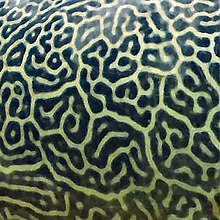
\includegraphics[width=0.6\textwidth]{220px-Giant_Pufferfish_skin_pattern_detail.jpg}
\end{minipage}
\begin{minipage}{0.5\textwidth}
\centering
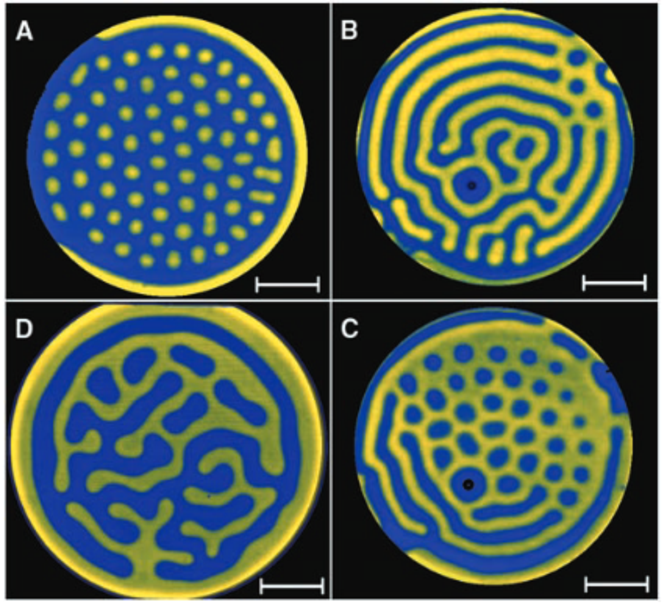
\includegraphics[width=0.7\textwidth]{turing_pattern_chem.pdf}
\end{minipage}
\caption{Motifs de turing sur la peau du poisson-globe, à gauche. A droite, motifs de turing émergeant d'une réaction chimique \cite{Horvth2009AnED}.}
\label{fig:turing_pattern}
\end{figure}

Qui dit système complexe dit système modulaire ?
Réseaux sociaux, communautés de fourmis, autant d'exemples montrant une emergence auto-organisée de modules. 


Système complexe adaptatif (cas) introduit par john Holland et Murray gellmann.
Ces systèmes sont un sous ensemble des systèmes complexes. Il s'agit de systèmes multi-agents qui réagissent à leur environnement, et s'auto-influencent. Ils se distinguent par l'émergence de propriétés et l'auto-organisation. C'est précisément ce qu'on cherche à faire dans un réseau de neurones. On dira qu'il y a eu un apprentissage si l'évolution du système a conduit à l'émergence de propriétés montrant une généralisation d'information sur les données présentées. 


%%%%%%%%%%%%%%%%%%%%%%%%%%%%%%%%%%%%%%%%%%%%%%%%%%%%%%%%%%%%%%%%%%%%%%%%%%%
% SECTION 1 introduction via la biologie, exemples 
%%%%%%%%%%%%%%%%%%%%%%%%%%%%%%%%%%%%%%%%%%%%%%%%%%%%%%%%%%%%%%%%%%%%%%%%%%%%






%%%%%%%%%%%%%%%%%%%%%%%%%%%%%%%%%%%%%%%%%%%%%%%%%%%%%%%%%%%%%%%%%%%%%%%%%%%%%
% SECTION 2 : définitions et propriétés
%- Tour d'horizons des définitions : en bio, en ingénieurie. Auto-organisation, conséquence de la modularité ? 
%- Taxonomie : fonctionnelle, stucture modulaire,emergence 
%- Position de l'autrice du manuscrit sur la modularité, intéret des différentes modularités
%- Discussion : est ce que notre esprit modulaire veut trouver de la modularité a tout prix ? ( quand la mod est fonctionnelle, peut etre biais de nos représentations ? Mais, on observe assez objectivement des modules physiques via les connexions dans de nombreux réseaux. Evolution l'a fait comme ca, probablement une réponse globale a un problème. 
%- Echelles de la modularité. 
%- Activation d'autres modules
%- Mutli-modalité - un mot, rappel dans une autre partie
%%%%%%%%%%%%%%%%%%%%%%%%%%%%%%%%%%%%%%%%%%%%%%%%%%%%%%%%%%%%%%%%%%%%%%%%%%%%%%%

\section{Quelle définition de la modularité ?}

L'étude de la modularité des systèmes est vaste. Entre étude des systèmes biologiques, ingénieurie des réseaux de neurones, ou même sociologie, les définitions de modularité varient. Nous chercherons donc dans cette partie à exhiber des définitions et des spécificités de ce qu'on appelle modularité.

\subsection{Modularité structurelle}

Lorsque le système possède une structure définie de réseau, typiquement un réseau de neurones, on peut définir une modularité en terme de graphe. Un système modulaire est ainsi \emph{Un système qui a une structure de graphe modulaire}.
Même en tant que graphe, modulaire est un terme large. De nombreux travaux proposent "une architecture modulaire" sans vraiement définir ce terme. 

\subsubsection{Mesurer la modularité structurelle d'un réseau}

La modularité d'un réseau est définie en théorie des graphes par le fait de pouvoir détecter des zones fortement connectées au sein de ce réseau, reliées par peu de connexions. Il s'agit donc de détecter des cliques, des sous-graphes fortement connectés, et de les différencier des zones moins connectées. 
La quantité la plus largement utilisée pour définir la	modularité d'un graphe est le \emph{coefficient de clustering}. Ce coefficient mesure la probabilité que deux noeuds soient directement connectés en sachant qu'ils ont un voisin en commun. Les réseaux sociaux par exemple, présentent des forts coefficients de clustering. D'autres mesures sont possibles, menant à une détection de zones fortement connectées. Cette modularité peut également se mesurer en regardant la densité des arêtes dans une partition du graphe, relativement à ce qu'on attendrait dans un graphe aléatoire. 

rich club -> ???

%\cite{Harriger2012RichCO}-> mesure modularité dans le cerveau, partie "méthodes" explique les méthodes de mesure de modularité. TODO les lister

\subsubsection{Réseaux en "petit-monde"}

La modularité d'un réseau est reliée à la propriété de petit-monde d'un graphe. 
Un graphe en \emph{petit-monde} (small-world network) est un graphe dans lequel la distance moyenne entre deux noeuds est proportionnelle à $\log(N)$, $N$ étant le nombre de noeuds du graphe. En d'autres termes, c'est un graphe dans lequel on trouvera forcément un chemin assez court relativement à la taille du réseau, entre n'importe quels noeuds. Un exemple typique de réseau en petit monde est celui des relations sociales avec la règle des "six degrés de séparation" mis en lumière par Stanley Milgram en 1967 \cite{Milgram1967TheSW} : en prenant deux individus au hasard aux états unis, Milgram montre qu'on peut les relier de connaissance mutuelle en connaissance mutuelle en, en moynenne, 6 étapes. Maintenant que la plupart de nos connaissances sont en enregistrées sur les réseaux sociaux, cette distance, entre tous les utilisateurs de facebook dans le monde entier, a été mesurée comme étant 3.5 degrés de séparation en 2016 \footnote{\url{https://research.fb.com/three-and-a-half-degrees-of-separation}}. La propriété de petit-monde est mesurée par le \emph{coefficient de petit-monde} $\sigma$. Il se mesure en comparant des métriques du graphe avec celles d'un graphe aléatoire équivalent, c'est à dire un graphe aléatoire ayant le même nombre de noeuds et la même densité de connexions. 
En notant $C$ le coefficient de clustering du graphe, $C_r$ celui d'un graphe aléatoire équivalent, $L$ la longueur (nombre d'arête) moyenne du plus court chemin entre tous les noeuds du graphe, et $L_r$ cette longueur dans un graphe aléatoire équivalent. 

$$\sigma = \frac{\frac{C}{C_r}}{\frac{L}{L_r}} $$

Un réseau est dit petit-monde si $\sigma > 1$, autrement dit, si la longeur du plus court chemin est inférieure à celle d'un graphe aléatoire, et/ou si le graphe présente plus de communautés qu'un graphe aléatoire. Cette métrique est cependant assez limitée, et il est plus judicieux existe d'autres mesures, comparant cette fois le coefficient de clustering et la longeur moyenne du plus court chemin à des graphes équivalents en treillis en plus des graphes aléatoires. 

Un réseau petit-monde n'est pas forcément modulaire. Par contre, un graphe ayant une structure modulaire, avec des communautés fortement connectées, est petit-monde. Un exemple est donné en figure~\ref{fig:graphe}. Le réseau $(b)$ est petit-monde : on trouve forcément un chemin court entre deux noeuds. Le réseau $(c)$ est également petit-monde, mais présente aussi des sous-graphes fortement connectés. 
La propriété de petit-monde semble avoir des avantages computationnel et se retrouve ainsi dans de nombreux exemples de réseaux biologiques. Nous détaillerons cet avantage en partie suivante. 

\begin{figure}
\centering
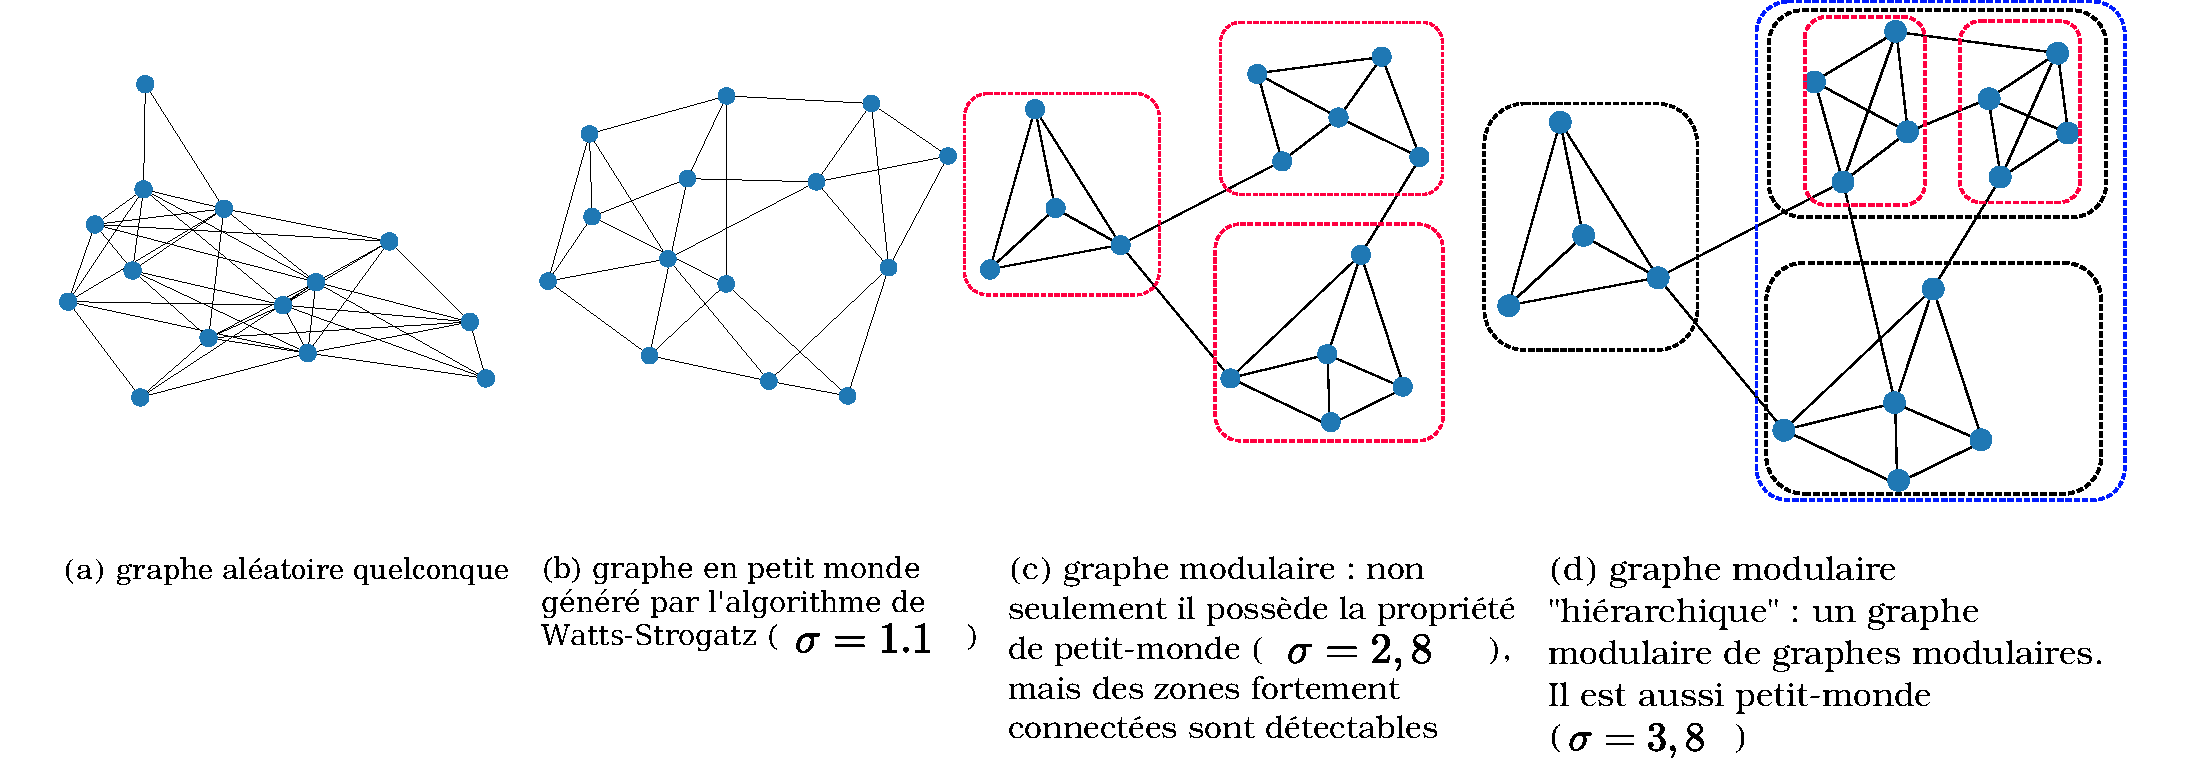
\includegraphics[width=\textwidth]{types_graphes.pdf}
\label{fig:graphe}
\end{figure}


\subsubsection{Modularité auto-similaire}

Si on prend un sous-graphe fortement connecté d'un graphe modulaire, ce sous-graphe peut éventuellement, à son tour, présenter une structure modulaire. On peut alors parler de modularité \emph{hiérarchique}, ou \emph{auto-similaire}. L'auto-similarité renvoie au processus de construction dans lequel on connecte par une arête deux structures jumelles (par exemple deux graphes complets); on copie ce graphe et on le connecte par une arête à sa copie pour former un graphe plus grand, etc. On gardera le terme auto-similaire pour parler de graphes formés de modules de modules, même si ces modules ne sont pas des copies exactes d'eux mêmes à différentes échelles, afin de garder le terme hiérarchique pour d'autre structures. Cette modularité "à différentes échelles" est souvent présente dans les réseaux. Le cerveau est par exemple souvent présenté comme un réseau modulaire auto-similaire \cite{Meunier2010ModularAH}. Des modules larges (aires fonctionnelles) sont formés de sous-modules, eux mêmes décomposables en sous-modules, etc. 

\subsubsection{Réseaux invariant par échelle}

Un dernier type de réseau à relier à la modularité sont les réseaux sans échelles (\emph{scale-free networks}). Un réseau small world est un réseau dont le nombre de noeuds de degré $k$ suit une loi de puissance. Les réseaux sans échelles ont notamment été étudiés par Barabasi lors de l'étude du world wide web, \cite{Barabasi2003ScaleFreeN}.
Ces réseaux sont "ultra-modulaires", ils ont un coefficients de clustering élevés. Il se caractérisent par la présence de sous-graphes ultra-connectés, mais connectés par un \emph{hub}, un noeud connectant d'autres noeuds moins connectés. Par leur distribution de connexions, on retrouve également dans ces réseaux une propriété d'auto-similarité: un sous-graphe autour d'un hub présentera une structure similaire à un sous-graphe plus grand, centré sur un plus gros hub, les hubs étant reliés entre eux. Par cette modularité, ils présentent donc aussi une caractéristique de petit-monde. Ces réseaux sont répandus au sein des structures sociales, par exemple les réseaux de citations entre articles scientifiques, les réseaux sociaux...

\subsubsection{Conclusion}


\cite{Hilgetag2015IsTB} : différencie réseaux small world et réseaux hiararchique modulaires, et statue qu'un réseau peut etre "hiérarchique modulaire" même s'il n'est pas small world, mais possède une dimension topologique finie. 
\cite{Meunier2010ModularAH} : statue que un réseau modulaire est small world,


En bref : 
- techniques de detection de communautés sur des graphes pour detecter une modularité.
- Certaines structures se distinguent parmi les graphes modulaires :  small-world, scale-free, hiérarchique. ces structures se recoupent.
- Au niveau du cerveau, on n'est pas hyper d'accord sur le type de modules, mais les expés montrent une structure. 
- Echelles des modularités, hyper important.
- Réseaux sociaux présentent aussi ces formes de modularité. 

\subsection{Modularité fonctionnelle}

La frontière est floue entre modularité structurelle et fonctionnelle. Les deux vont probablement de pair, mais parfois un système ne présente pas de structure de graphe visible, et l'étude de sa connectivité n'est pas possible. L'étude de ce système passe alors par les fonctions qu'il met en jeu : alors, une partie du système répondant à une fonctionnalité particulière sera considérée comme un module du système. 


\subsection{Modularité temporelle}

Du point de vue du système dynamique, l'aspect temporel n'est finalement qu'une dimension de plus dans la modularité du système. Les règles locales faisant évoluer le système dynamique amènent à des comportements complexes temporellement parlant. Par exemple, un attracteur fractal est le résultat des trajectoires d'un système dynamique complexe à l'état de chaos. 

La modularité s'associe aux séquences dans le cerveau. Les mémoires, l'interaction entre échelles de fonctionnement apportent une modularité supplémentaire.

\subsection{Modularité émergente ou modularité définie}

\subsection{Emergence d'une modularité et auto-organisation}

Est ce que l'auto-organisation d'un système dénote d'une modularité ? 


\section{La modularité, répandue dans les système biologiques}

% Passer cette partie après la section définition ???
\subsection{Le cerveau, réseau modulaire fondamental}

Un neurone est un système dynamique, donc l’activité electrique est régie par des équation d’évolution dépendant des connexions qu’il recoit. Le cerveau dans son ensemble est alors,  fondamentalement, un agrégat de neurones. 300 neurones dans le ver microscopique  Caenorhabditis elegans, un million dans le cerveau des insectes, jusqu’a 86 millards de neurones dans un cerveau humain. Tous ces pics electriques et chimiques nous permettent une prise de décision, une mémoire, de la réflexion, des représentations …. Un ensemble de capacités que l’on nomme intelligence. Cette intelligence n’est pas localisée dans le cerveau, de ce qu’on sait. Elle résulte de l’activité globale de l’ensemble de neurone, et est ainsi une propriété émergente. 

Cet amas obscur est le point de départ des études autour de l’intelligence artificielle. Si on veut créer un systèmes ayant une intelligence émergente, il nous faut comprendre les mécanismes de cette émergence, et donc comprendre les systèmes existant ayant cette capacité. Les réseaux de neurones se sont donc d’abord inspirés du cerveau avant d’être développés plutot sur un aspect computationnel avec moins de vraisemblance biologique.
Cette inspiration biologique ne se limite pas à assembler des neurones : l’architecture cérébrale à plus grande échelle est aussi une source d’inspiration dans la recherche de systèmes intelligents, autrement dite, intelligence artificielle.  
Et le cerveau semble avoir une architecture particulière : il est modulaire, à plusieurs échelles. 
Les premières propositions de modèle du cerveau humain datent du début du XXeme siècle. Déjà, un découpage en aires est proposé pour expliquer le fonctionnement de cet organe, notamment avec les travaux de Broca et Wernicke qui mettent en lumière des zones du cerveau qui semblent responsable du langage. Le modèle connexioniste du cerveau, formalisé à partir de ces travaux par Geschwind dans les années 60 , décompose ainsi le langage en plusieurs fonctions : la compréhension, la lecture et l'action de parler. Ce modèle n'est plus vraiment utilisé, mais l'idée de décomposition en modules reste valable.
Avec l'avènement des outils d'imagerie, le cerveau a pu être cartographié plus préciséement en un ensemble d'aires, agissant comme modules fonctionnels au sein d'une structure complexe; ces aires sont elles mêmes composées de modules distincts. 

L'étude des aires et des connexions entre zones du cerveau, comme~\cite{primate_cortex_91} dans le cas du cortex visuel du primate, découpent les zones activée pour la vision en modules distincts, et montrent que ces modules sont connectés. Ces connexions, en fonction des modules, sont réciproques ou non. Les "pathsways" du cerveau désignent des modules fortement connectés. Leur détection expérimentale est réalisée en relevant des indicateurs de dépendance (corrélation, ..., en fonction des méthodes utilisées). Ainsi, \cite{Rolls2002ComputationalNO} précise la structure des différentes aires cérébrales en présentant les connexions au sein de ces aires, par exemple la structure présentée en figure~\ref{fig:cortex2} pour l'aire visuelle. 
Les connexions du cerveau sont présentes à différentes échelles: des pathsways existent ainsi au sein de l'aire visuelle du cerveau, mais des boucles de rétroaction entre zones cérébrales sont présentes à plus grande échelle, par exemple la boucle baso-thalamo-corticale. Ces différentes échelles au sein du cerveau amènent \cite{Meunier2010ModularAH} à le présenter comme un réseau "hiérarchique modulaire". Cette activité "sans échelle" pourrait notemment permettre au cerveau d'appréhender les notions temporelles, transposant ainsi un réseau spatial en une activité temporelle \cite{biyu_scale-free_2014}.

La structure cérébrale est donc bien particulière. Aussi, l'inspiration cérébrale des modèles d'intelligence articielle ne se résume pas au modèle neuronal, les éléments architecturaux et de connexions sont donc à considérer. 
\begin{figure}[t]
\centering
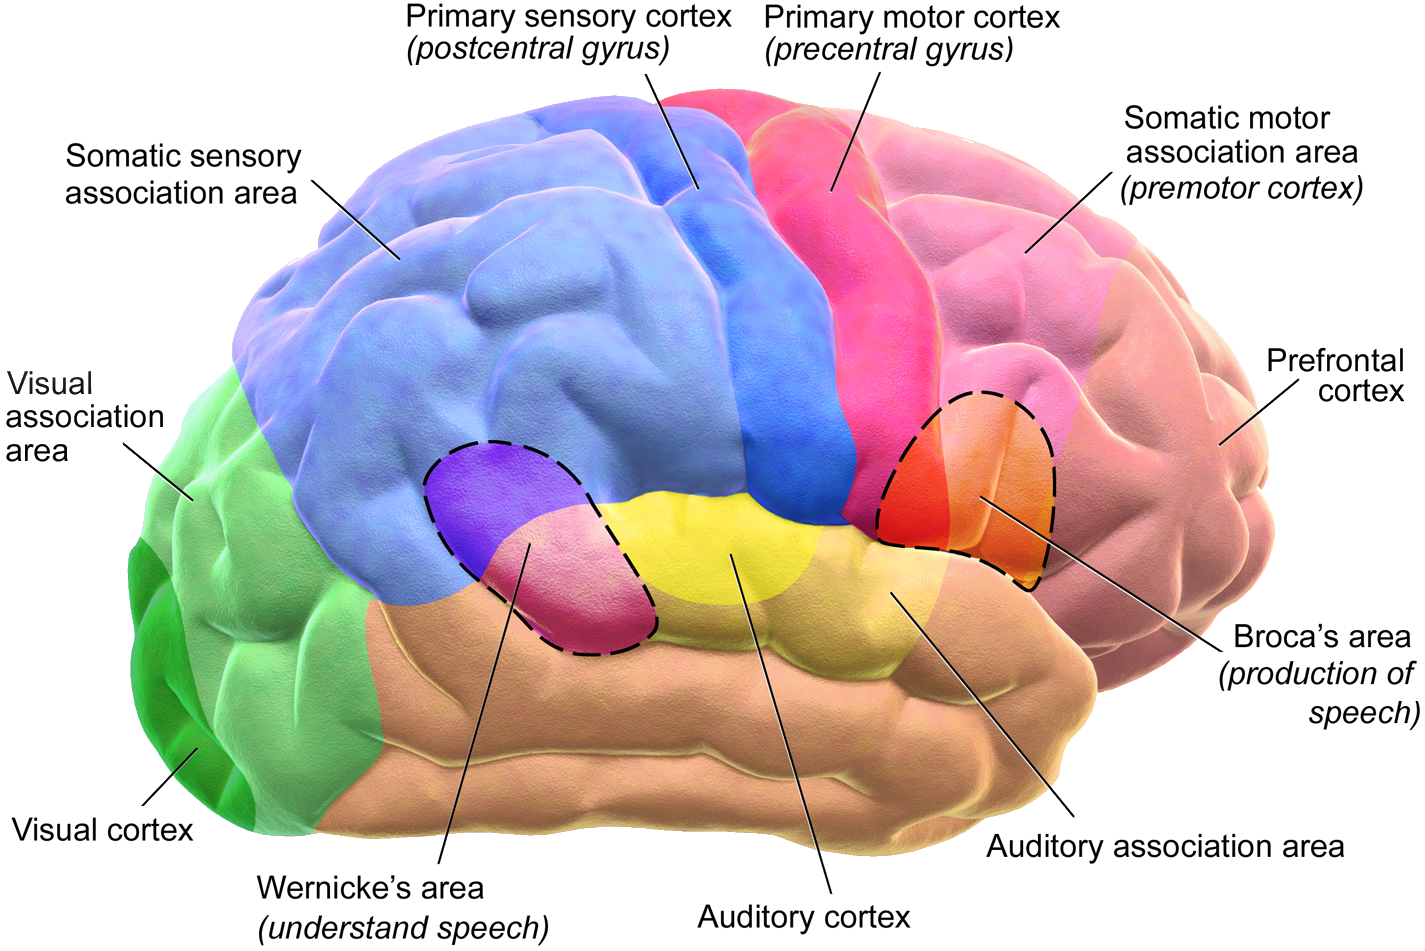
\includegraphics[width=0.5\textwidth]{Blausen_0102.png}
\caption{Aires du cerveau humain}
\end{figure}

\begin{figure}[t]
\begin{minipage}{0.5\textwidth}
\centering
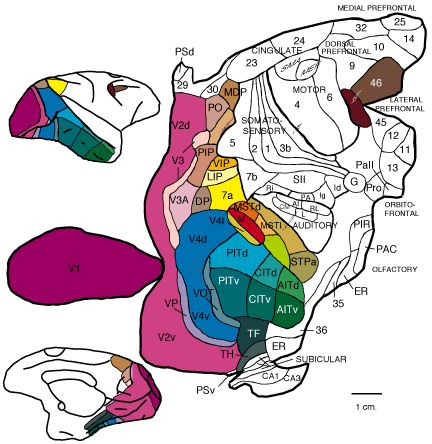
\includegraphics[width=0.7\textwidth]{FVE_fig2map.png}
\label{fig:cortex1}
\end{minipage}
\begin{minipage}{0.5\textwidth}
\centering
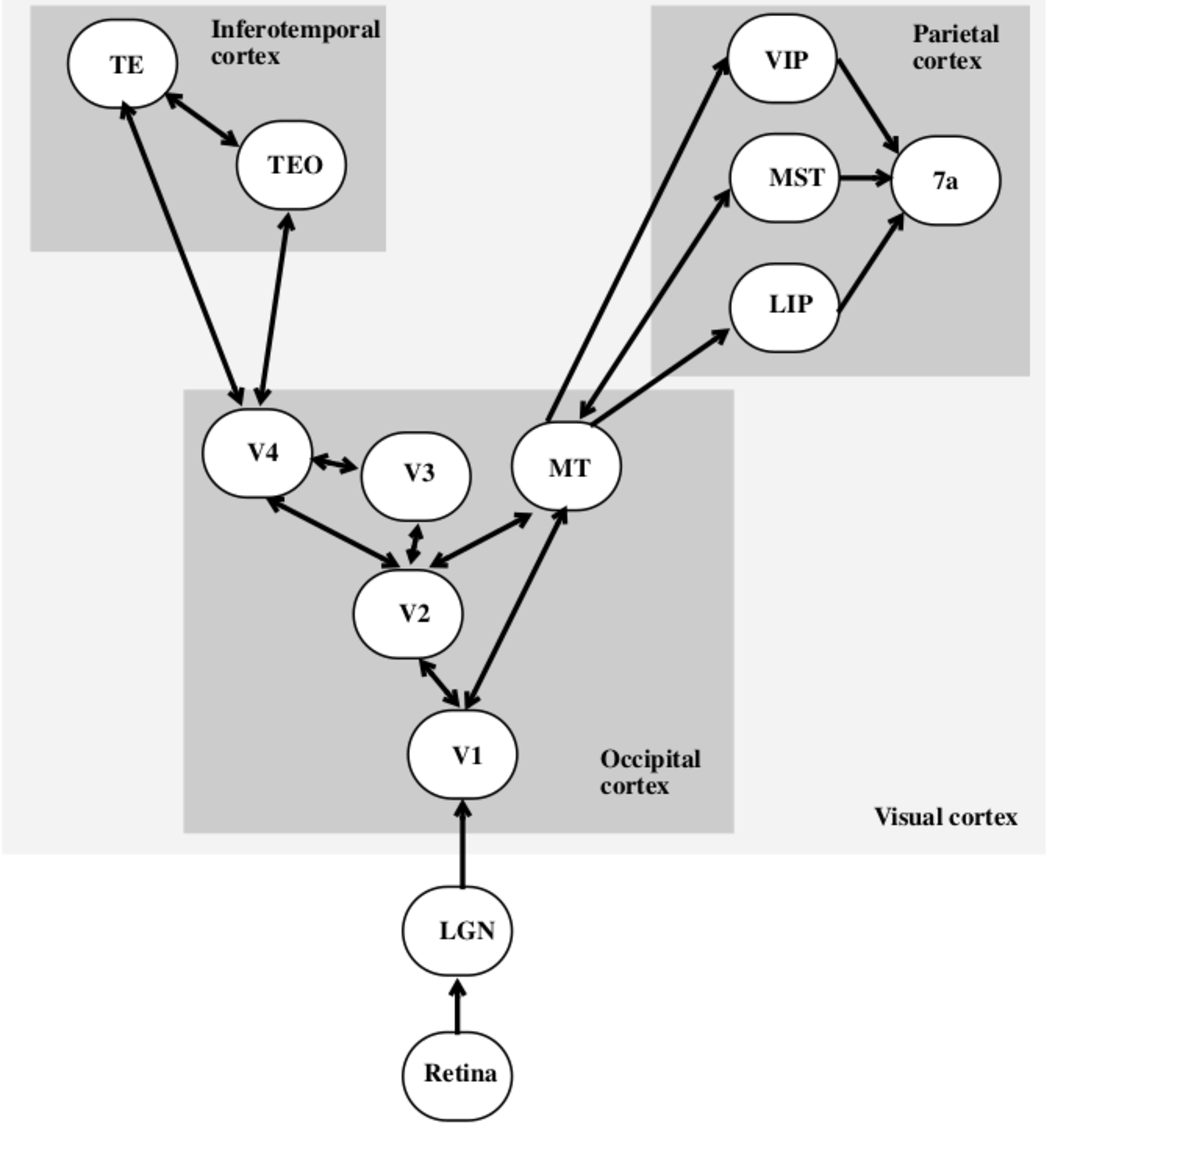
\includegraphics[width=0.8\textwidth]{rolls_pathways.pdf}
\label{fig:cortex2}
\end{minipage}
\caption{carte aplanie des aires du cortex visuel du macaque \cite{primate_cortex_91}, à gauche, et pathways dans ce cortex visuel entre les aires à droite \cite{Rolls2002ComputationalNO}. L'architecture neuronale présente des rétroaction entre zones, dans une architecture non-hiérarchique.}
\end{figure}

 
%- Nombreuses études s'appuient sur le système modulaire : le cerveau \cite{primate_cortex_91,mountcastle_columnar_1997,binzegger05}
%
%
%- Modularité hiérarchique( modules de modules) -> Ajouter infos depuis l'article qui parle de modules hiérarchiques. 
%%Ajouter figure du cerveau avec le schéma des aires
%
%Finalement : 
%Cerveau présente ce qu'on peut appeler des modules, avec des connexions entre eux, avec rétroaction. 
%
%Leur mesure peut etre structurelle (regarder les structures de neurones), ou fonctionnelle : quelles aires s'activent pour une fonction ? \\
%Détail des types de modularité en parties suivantes. 

\subsection{Des réseaux et des modules dans tous les systèmes biologiques}

Les phénomènes émergents ne se limitent pas au cerveau : tous les systèmes biologiques semblent présenter des fonctionnement issus de systèmes complexes, menant à une régulation globale d'une quantité, à un comportement commun, autrement dit, l'émergence d'un comportement. On peut par exemple citer l'exemple des nuées d'oiseaux : des centaines ou des milliers d'oiseaux peuvent voler ensemble, sans se heurter ni se disperser, le tout sans avoir d'instructions globale. Cette capacité à rester en nuée émergent des règles locales que connaissent chacun des oiseaux. Ces règles régissent le comportement individuel à avoir avec leur voisins proches. Ces règles simples permettent à ces milliers d'individus de voler en groupe et de se déplacer.
Les arbres en forêt s'adaptent, pour pousser sans se toucher, et partageraient même des information en communiquant. Sans forcément parler d'intelligence, on peut tout à fait voir en ces comportement des mécanismes émergents. Le blob, 

%%%%%%%%%%%%%%%%%%%%%%%%%%%%%%%%%%%%%%%%%%%%%%%%%%%%%%%%%%%%%%%%%%%%%%%%%%%%%%%%%%%%%%%%%%%%%%%%%%%%%%%%%%%%%%%%%%%%%%%%%%%%%%%%%%%%%%%%
% SECTION 3: quel intéret à utiliser des architectures modulaires pour l'apprentissage ? 
% - 
%%%%%%%%%%%%%%%%%%%%%%%%%%%%%%%%%%%%%%%%%%%%%%%%%%%%%%%%%%%%%%%%%%%%%%%%%%%%%%%%%%%%%%%%%%%%%%%%%%%%%%%%%%%%%%%%%%%

\section{Intérêt computationnel des réseaux modulaires}

Barabasi : Hypothèse que les réseaux small world présentent un avantage evolutionnaire.
Modularité hiérarchique présente l'avantage de maintenir une activité dans le réseau sans que ca ne colonise tout ni ne s'eteigne, ce qui est nécessaire pour la computation. 

\subsection{Modularité, complexité et émergence d'un apprentissage ? }

Systèmes complexes et emergence: possibilité d'apprentissage, exemple du reservoir computing

La modularité est liée a la complexité des systèmes, donc l'emergence de comportements chaotiques et/ou synchronisés. 

SYSTEMATIC GENERALIZATION : WHAT IS REQUIRED
AND CAN IT BE LEARNED ? : 
Our findings show that the generalization of modular models is much more systematic and that it is highly sensitive to the module layout, i.e. to how exactly the modules are connected.

Simplicité de la modularité : exemple de construction des fractales, exemple du rigaudon

Parler des architectures de Hebb (précurseur) ici ou avant ?

\subsubsection{réponse a un problème de contrainte physiques, énergétiques}

- Parallelisme, calcul et small world networks : réponse a un problème de contrainte physiques, énergétiques. 
- Calcul distribué 
- Automates cellulaires  ?

- Exemple des puces neuromorphiques, calcul embarqué


Conclusion: En décentralisant le calcul, on cherche aussi à plus facilement l'utiliser via des architectures neuromorphiques. 


\subsection{Types de connexions}

Opaque vs tout savoir

 
%%%%%%%%%%%%%%%%%%%%%%%%%%%%%%%%%%%%%%%%%%%%%%%%%%%%%%%%%%%%%%%%%%%%%%%%%%%
% SECTION 4 En pratique, ou en est on des réseaux de neurones modulaires ?
%%%%%%%%%%%%%%%%%%%%%%%%%%%%%%%%%%%%%%%%%%%%%%%%%%%%%%%%%%%%%%%%%%%%%%%%%%%%%ùù

\section{Modularité dans les réseaux de neurones}

Au sein des systèmes complexes, les réseaux de neurones artificiels se sont directement développés en s'inspirant des réseaux biologiques. Hebb formule ainsi en 1949 "neurons that fire together, wire together". Les réseaux de neurones développés depuis sont alors inspirés de la biologie, en s'en éloignant plus ou moins. Quel que soit leur éloignement, ce sont des systèmes complexes dans le sens ou il s'agit d'un grand nombre de neurones reliés entre eux, et qu'on développe dans le but de l'émergence d'une propriété d'apprentissage et de généralisation.

Ces réseaux sont par exemple le perceptron, les cartes auto-organisatrices. 
L'intérêt de chercher des aspect modulaires des réseaux de neurones a été formulé par exemple par \cite{towards_novel_2001} : 

A partir du perceptron, les réseaux de neurones profond ont été développés comme une assemblée de perceptrons reliés hiérachiquement (fin 90 ) 

\subsection{Deep Learning}
Boites noires qui ont des performances remarquables sur tous les domaines, leur représentation et compréhension est quant à elle toujours un challenge. Ajouter un aspect modulaire non-hiérarchique dans les calculs de ce genre de réseau, pour augmenter la vitesse d'apprentissage ou encore pour 

\subsubsection{Réseaux de neurones profond et modulaires}

- Réseaux qui apprennent a s'organiser en modules. Interet. Limites ? Performances ? \cite{Andreas2016NeuralMN,Kirsch2018ModularNL}
"The NMN approach is intuitively appealing but its
widespread adoption has been hindered by the large amount of domain knowledge that is required
to decide (Andreas et al., 2016) or predict (Johnson et al., 2017; Hu et al., 2017) how the modules
should be created (parametrization) and how they should be connected (layout) based on a natural
language utterance. Besides, their performance has often been matched by more traditional neural
models" ( systematic generalization article ) 

\subsubsection{Utiliser des modules pour mieux représenter les réseaux de neurones profond}
- Trouver des modules dans les réseaux pour les expliquer ? \cite{Watanabe2018ModularRO,Csordas2021AreNN}
are neural net modular : "it uses different modules for very different functions = Pspecialize," et "it uses the same module for identical functions that
may have to be performed multiple times = Preuse"
- Reconciling deep learning with symbolic artificial intelligence: representing objects and relations(2019)
Pb du deep learning = Data inefficiency (comparé a l'humain);Poor generalisation; Lack of interpretability.

\subsection{Réseaux auto-organisés}

Les réseaux auto-organisés sont directement inspirés des réseaux biologiques. Au sein de ces réseaux
Plus qu'en deep learning, les réseaux de neurones auto-organisés
- Auto-organisation prend une profonde inspiration biologique, tout comme les modules.
- Exemple de réseaux auto-organisés modulaires : développer dans la partie suivante.
\begin{figure}
\begin{minipage}{0.5\textwidth}

%\centering
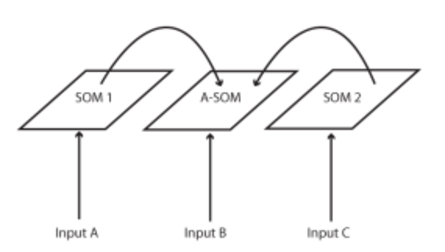
\includegraphics[width=\textwidth]{asom}
\caption{A-SOM model \cite{johnsson_associative_2009}}
\end{minipage}
\begin{minipage}{0.5\textwidth}
%\centering
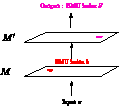
\includegraphics[width=0.9\textwidth]{hsom}
\caption{HSOM model \cite{LampinenClusteringPO}}

\end{minipage}
\end{figure}
\cite{LampinenClusteringPO}

\cite{parisiLL}

Lefort

Travaux préliminaires de l'équipe ->  Bassem, Ménard ?



\subsection{Construire une architecture modulaire}

A mettre dedans : 

- Réseaux top down / modulaires ? définition, a quel point un réseau est modulaire, qu'est ce qu'on appelle réseau modulaire ? 
Fonction définies au préalable vs émergence des fonctions. 
Modules définis au préalable vs émergence des modules. 


%%%%%%%%%%%%%%%%%%%%%%%%%%%%%%%%%%%%%%%%%%%%%%%%%%%%%%%%%%%%%%%%%%%%%%%%%%%%%%%%
% SECTION 5 : proposer des enjeux par rapports au réseaux listés précedemment 
%%%%%%%%%%%%%%%%%%%%%%%%%%%%%%%%%%%%%%%%%%%%%%%%%%%%%%%%%%%%%%%%%%%%%%%%%%%%%%%%


\section{Enjeux d'une architecture modulaire de SOMs}

On connait plutot bien les SOM, mais on sait que des comportements nouveaux peuvent émerger lorsqu'on met en interaction des systèmes étudiés séparément. 
On peut donc se poser la question des comportements qui peuvent survenir dans ce cas.

Dans les structures de cartes étudiés, modularité forte dans le sens ou les fonctions des modules sont prédéfinies. Si on ne fournit que les règles d"interaction, ou est ce qu'on se situe ? 
 
 
Position du manuscrit : architecture 
%%%%%%%%%%%%%%%%%%%%%%%%%%%%%%%%%%%%%%%%

Plan de la partie ! 

 

\begin{enumerate}
\item Intro : Notre monde est modulaire, en tout cas nous l'interprétons en tant que tel. Proposé déjà dans les années 60 - breve histoire des réseaux de neurones ?
Remarquer que nous, observeur, raisonne et se construit modualairement. Il nous est difficile de concevoir les choses autrement. 
Les disciplines sientifiques par ex, un domaine obéit a des principes
\item Qu'appelle t-on la modularité ? Définitions claires et propriétés
	\begin{itemize}

		\item Definition
			\begin{enumerate}
			\item Structurelle, dans les systèmes réseaux
			\item Fonctionnelle, dans les systèmes dont on ne connait pas la structure ?\\
			\item Temporelle / mais est ce que le temps ce n'est qu'une dim de plus
			\item Modularité hiérarchique attention : deux defs a hiérarchiques. Soit c'est une histoire de connexions, soit d'auto-similarité. On parle nous de l'auto similarité !!! Au contraire l'autre forme de hiérarchie n'est pas observée en bio.
			\end{enumerate}
		
		\item Propriétés de la modularité 
			\begin{enumerate}
			\item Auto-organisation
			\item Types de connexions
			\item Emergence
			\end{enumerate}
	\end{itemize}	
\item Exemples Biologiques et computationnels
	\begin{enumerate}
	\item Biologie : opti evolution a priori...
	\item Computationnel : pareil.
	\end{enumerate}
	
\item Maintenant qu'on sait ce que sont les systèmes modulaires, en quoi on peut faire de l'apprentissage avec ? Quels sont les intérêts ?
	\begin{enumerate}
		\item Exemples de réseaux auto-organisés
		\item Exemples de réseaux de neurones : deep learning
	\end{enumerate}

\end{enumerate}





